\documentclass[11pt]{article}
% for \begin{center}, etc.
\usepackage{geometry}
% all kinds of math macros
\usepackage{amsmath}
\usepackage{amssymb}
% eps figures
\usepackage{epsfig}
% drawing trees
\usepackage{tikz}
%colors
\usepackage{color}
\definecolor{light-blue}{rgb} {0.8,0.8,1.0}
\usetikzlibrary{trees,positioning}
%code listings
\usepackage{listings}
\lstset{frame=single,
        basicstyle=\footnotesize}
% Margins
\usepackage{fullpage}
\newcommand{\ben}{\begin{enumerate}}
\newcommand{\een}{\end{enumerate}}
\newcommand{\bit}{\begin{itemize}}
\newcommand{\eit}{\end{itemize}}

\newcommand{\AR}{{\tt AmrRegion}}
\newcommand{\AL}{{\tt AmrLevel}}
\newcommand{\MF}{{\tt MultiFab}}
\newcommand{\BA}{{\tt BoxArray}}
\newcommand{\DM}{{\tt DistributionMapping}}

\begin{document}

\title{Technical Report for the Region-Based AMR version of BoxLib}
\author{Ethan Van Andel \\ UCB, LBNL}

\maketitle

\begin{figure}[h]
\centering
\includegraphics[width=\textwidth]{regions-logo.png}

\end{figure}

\newpage
\tableofcontents
\newpage

\section{Introduction}

This document provides an introduction to the Region-Based model of 
AMR (RAMR) 
as implemented in BoxLib. This document assumes that the reader is 
familiar with traditional AMR and the basic structure of BoxLib. The 
primary intended audience is programmers and scientists who work with 
BoxLib and want to get started in the RAMR version and/or 
transfer existing traditional codes to the RAMR version.

\subsection{Region-Based AMR}
Traditional AMR treats all grids at a single level of refinement as a 
single conceptual entity, a ``level'' (\AL{}). All grids at the level are 
advanced together with a single timestep. 

RAMR breaks down a level into multiple ``regions'' (\AR{}). All regions at a 
given level have the same spatial refinement but may have different 
timesteps and may be advanced independantly. Where traditional AMR 
organizes its levels in a "Tower" with finer levels contained in 
coarser ones, RAMR is structured as a "Tree" with multiple fine 
child regions contained in a single coarse parent.

RAMR's primary advantage is the ability to reduce time spent advancing 
grids with unnecessarily small timesteps. Using the technique of 
Optimal Subcycling (\ref{subcycling}), each region chooses the 
best possible timestep. For example, in a traditional AMR simulation, 
a small, portion of the domain dictates the timesteps over the entire 
domain. In RAMR simulations, that portion can be isolated in a single 
region and advanced with multiple small timesteps while the rest of 
the domain takes larger steps.

\subsection{Overview}

The rest of is document is organized as follows. Section \ref{concepts} 
describes the main concepts and data structures introduced 
in the RAMR version of BoxLib. The following section, \ref{changes}, 
discusses other key changes to BoxLib. Readers interested in 
converting existing codes to the RAMR model should consult 
section \ref{transition} which details the changes that need to be 
made, both to run in the RAMR code as a traditional AMR simulation, 
and to transition fully to the RAMR model. The final section, 
\ref{future}, discusses additional applications and planned 
capabilities for the RAMR code.

For coding purposes, the following section should be viewed as a 
high-level companion to--not a replacement for--the in-code 
documentation. The non-coding reader will be able to obtain a general 
understanding of the key new concepts and changes necessary for 
Region-based AMR.


\section{Central Concepts}
\label{concepts}

RAMR simulations introduce new algorithmic and structural concepts to 
traditional AMR. This section provides a high level overview of those 
concepts. The \AR{} (\ref{amrregion}) class replaces \AL{} as the 
central structure in RAMR simulations. Regions and associated data are 
stored in tree data structures (\ref{trees}) that provide a number of 
methods for controlling RAMR simulations. Some operations such as 
regridding or multilevel solves may make use of data from more than 
one \AR{} in a level of refinement. These operations make use of 
aggregation (\ref{aggregation}) methods to allow them to treat 
multiple regions as one for their purposes. Finally Optimal Subcycling 
(\ref{subcycling}) allows regions to choose their timesteps to 
maximize simulation efficiency.

\subsection{AmrRegion}
\label{amrregion}
The \AR{} is the new fundamental structure of BoxLib simulations. For 
most purposes, and \AR{} is simply a renamed \AL{}. Almost all methods 
from the latter are present and identical in the former. There are 
only a few key differences concerning the more complex tree structure 
of RAMR simulations. \AR{}s contain pointers to coarser regions, 
and have a unique ID that identifies them from other regions in the 
simulation (including those at the same level of refinement). These 
changes are minimal; the real differences appear in the data 
structures and  methods that act on \AR{}s.

\AR{}s obey the same nesting restrictions as \AL{}s; a fine region 
must be properly nested within the coarse region that contains it. 
Regions at the same level of refinement  may never overlap. In 
addition, the current code does not allow these regions to touch, but 
this is a temporary restriction and should be relaxed in future 
versions.

\subsection{Trees}
\label{trees}

Many {\tt Array}s and {\tt PArray}s in traditional BoxLib have been 
replaced by {\tt Tree}s and {\tt PTree}s. Tree data structures are 
used to store data that is \emph{stored globally} but \emph
{associated with a specific region}. This includes {\tt amr\_regions} the 
master tree of \AR{}s (formerly the array {\tt amr\_levels}) and control 
data structures such as {\tt n\_cycle} as well as application specific 
data such as particle storage and the gravity data for Nyx.

\subsubsection{Structure}
Trees are organized as traditional pointer tree data structures and 
can be represented as directed, rooted tree graphs. 
Trees are comprised of nodes, each of which contains pointers to its 
parent node and each of its children as well as data of some sort. 
Every tree has a single root node ($n_0$) with no parent. For the master 
tree of \AR{}s, the root node is the single region at refinement 
level 0 and the children of each node $n$ store the regions %that's awkward
at the next level of refinement contained in the region stored by $n$. 

{\tt Tree}s and {\tt PTree}s, like {\tt Array}s and {\tt PArray}s 
provide the essentially the same functionality, except that a {\tt 
PTree} stores pointers and can manage the associated memory.

\subsubsection{IDs}
Nodes in a tree are indexed by ID. An ID is an array of integers 
representing the node's position in a tree. The root node always has 
the ID $[0]$ while each the ID of each child node $n$ is the ID of 
$n_p$, followed by the index of $n$ among the children of $n_p$. An 
example of ID's can be seen in Figure \ref{id-example}.

\begin{figure}
\center
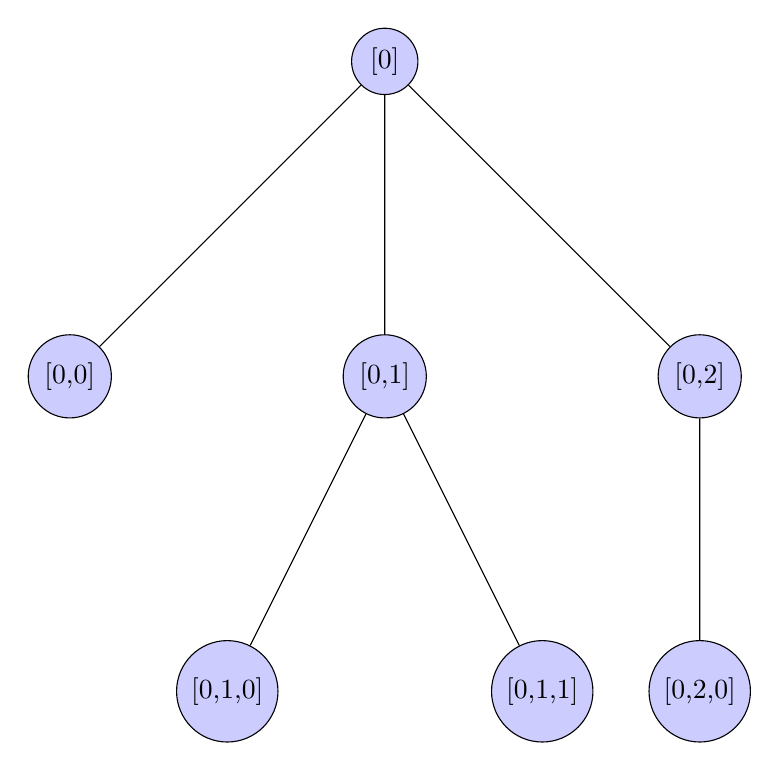
\begin{tikzpicture}[level 1/.style={sibling distance=4cm, level distance = 4cm}]
    \tikzstyle{every node}=[draw,circle,fill=light-blue]
    

    \node {[0]}
        child { node {[0,0]} }
        child { 
            node {[0,1]} 
            child { node {[0,1,0]} }
            child { node {[0,1,1]} }
            }
        child { 
            node {[0,2]} 
            child { node {[0,2,0]} }
            }
    ;
\end{tikzpicture}
\caption{An example tree with node IDs}
\label{id-example}
\end{figure}

For convenience and clarity, IDs in BoxLib are members of the {\tt 
ID} class. {\tt ID} is a derived class of {\tt Array<int>} 
that provides a few extra convenience methods. 

\subsubsection{Terminology}

In the remainder of this document will use the following 
terminology. The ``ancestors'' of node $n$ are the nodes in the path 
between $n$ and $n_0$. The ``descendents'' of $n$ are all nodes $n_d$
such that $n$ is an ancestor of $n_d$. In Figure \ref{id-example}, 
the descendents of [0,1] are \{[0,1], [0,1,0], [0,1,1]\} while the 
ancestors are \{[0], [0,1]\}. Note that n is considered to be among 
its own ancestor and among its own descendents. The ``siblings'' of 
$n$ are all of the children of the parent node $n_p$ of n. 
``Cousins'' are all nodes at the same level of the tree as $n$, or 
more technically, nodes the same distance from the root. [0,1,0] is a 
sibling of [0,1,1] while [0,2,0] is a cousin.

We will typically ignore the term node and simply use these terms in 
relation to the data stored by the nodes. For example, all \AR{}s 
are descendents of the singe coarse region. The union of the cousins 
of a given \AR{} contains all grids at that level of refinement. The 
descendents of $n$ can also be referred to as the ``subtree'' rooted 
at $n$

\subsubsection{Access and Iterators}
\label {iterators}

Nodes themselves are protected members of a tree. Outside methods 
only deal with the data and overall structure. Data in a tree can be 
accessed directly, or by use of iterators. Direct access works by 
way of ID, for example:
\begin{lstlisting}[backgroundcolor=\color{light-blue}]
    Tree<std::string> myTree;
    ... build the tree here ...
    ID region_id(3);
    ID[1] = 2;
    cout << region_id;
    \\ prints "0_2_0"
    myTree.setData(region_id.parent(), "new parent string");
    cout << myTree.getData(region_id);
    \\ prints (for example) "original child string"
\end{lstlisting}

{\tt TreeIterator}s (and {\tt PTreeIterator}s) allow users to iterate 
over all nodes in a tree. Many AMR operations that were done by 
looping over levels are now done by using tree iterators to iterate 
over regions. There are many ways to adjust the behavior of iterators. 
Iterators can operate on the tree in Prefix ordering (where the 
iterator points to the parent node before pointing to the children), 
or in Postfix (the default) ordering (where the iterator points to the parent after 
pointing at all the children). Iterators can also be created to loop 
over a subtree rooted at a given node. Finally, iterators can be 
restricted to a specific level of the tree, thus pointing to a set of 
cousins within the tree (or subtree). Example uses of iterators can 
be seen in the following example.
\begin{lstlisting}[backgroundcolor=\color{light-blue}]
    Tree<int> myTree;
    ... build the tree here ...
    // print all nodes of the tree at level 2
    TreeIterator<int> it = myTree.getIteratorAtRoot(2);
    for( ; !it.isFinished(); ++it)
        cout << "Node " << it.getID() << " has value " << *it << "\n";
    ID base_id(2);
    // Iterate over the subtree rooted at [0,0] in prefix order.
    it = myTree.getIteratorAtNode(base_id, Prefix);
    for( ; !it.isFinished(); ++it)
        *it += 1;
\end{lstlisting}

Note that tree iterators don't follow the {\tt begin()} and {\tt 
end()} conventions common to many iterators.

\subsubsection{Structure Synchronization}

The ``structure'' of a tree refers to the organization of nodes within 
the tree, but is independant of the data stored by the nodes. An RAMR 
simulation uses a number of trees to store different types of data. It 
is necessary that all those trees have the same structure so that if 
the ID [0,2,1] refers to region $r$ in {\tt amr\_regions}, it also 
refers to the dt associated with $r$ in {\tt dt\_region}. To allow 
structures to be synchronized, trees can output a list representing 
their structure. Other trees can rebuild themselves based on that 
list. This can likewise be done for subtrees.

\subsubsection{ExecutionTrees}

In rare cases (for instance partial multilevel advances), it is 
necessary to perform some operation over only some descendents of a 
given node. This can be accomplished by created an {\tt 
ExecutionTree}, a special type of {\tt Tree} that can be configured to 
iterate over only part of its nodes.

\subsection{Aggregation}
\label{aggregation}

While many RAMR operations work logically on a region-by-region basis, there are 
some operations that are inherantly level-based. Multilevel elliptic 
solves are the primary example; if one is performing a multilevel 
solve from a given base region, it must be done over all descendents 
simultaneously, not broken up by region. In addition, there are 
situations such as plotting and regridding where one wants to be able 
to draw on all data at a level without regard to what region it 
belongs to. 

RAMR BoxLib uses aggregation methods to handle these situations. These 
aggregation methods create a new \AR{} or \MF{} from a list 
of \AR{}s or {\tt MultiFab}s at a given level. The \MF{}s 
that result from this operation are shallow; their {\tt FabArray}s 
contain pointers to the original FABs, rather than creating new data. 
This means that not only is the aggregate \MF{}created with minimal 
data transfer, but modifications to the data in the aggregate 
\MF{} are automatically reflected in the original components. This 
type if aggregation is referred to as direct aggregation.

There are also situations that require aggregate \MF{}s to store 
data that doesn't exist yet. These \MF{}s typically store 
intermediate data for multilevel solves, or derived data for 
plotting. This type if aggregation is referred to as indirect 
aggregation. Indirectly aggregated \MF{}s can be created from \BA{}s 
as normal, but must also be supplied with the proper \DM {}. 

By using these aggregation methods, it is possible to make all 
existing multilevel solves ``just work'' with no rewrites in the 
underlying numerics.

\subsubsection{DistributionMappings}
\label{distribution}

By default, \DM{}s are strictly associated with the number of boxes 
in a \BA{}. However, this paradigm is not reliable when 
dealing with aggregation. For instance, when one aggregates a pair of 
\MF{}s with 4 and 5 boxes respectively, the resulting \MF{} must have 
a \DM{} that accurately places each FAB on its original 
processor. However, that \DM{} is not necessarily the same as the 
\DM{} created for a general 9 box \MF{}. The direct aggregation 
methods create the desired \DM{}s automatically. However, since 
creating a \MF{} from a given \BA{} uses the general \DM{}, 
indirectly aggregated \MF{}s must be created with both a \BA{} and a 
correct \DM{}.

As RAMR BoxLib evolves, this paradigm may change further to allow for 
greater control of region parallelism.

\subsection{Optimal Subcycling}
\label{subcycling}

%this could be cleaned up later

Optimal Subcycling automatically chooses the best allowable timestep 
for each region. Each region $r$ subcycles $n_r$ times relative to 
its parent (where $n_r >= 1$). Thus after $n_r$ subiterations, $r$ and 
$r_p$ are again synchronized. This $n_r$ is selected for each region 
as a solution to a global constrained optimization problem that finds 
the subcycling pattern that maximizes the ratio between coarse dt and 
work required to advance one coarse timestep while respecting timestep 
restrictions at each level.


\section{Important Changes}
\label{changes}
In addition to the new concepts, RAMR features some important 
modifications to existing methods and data structures.

\subsection{Timestep}

The RAMR timeStep method is nearly the same as the traditional 
version. The key difference is in the process for advancing finer 
grids. The traditional timeStep advances a coarse level $l$ by 
$dt_l$, then recursively timesteps $l + 1$ $n_{l+1}$ times with 
$dt_{l+1} = dt_l/n_{l+1}$.

%this paragraph is clunky

RAMR timeSteps advance regions rather than levels. A timeStep call 
on region $r$ will advance $r$ by $dt_r$. It will then iterate over 
each child $r_{ci}$ of $r$, timeStepping $r_{ci}$ $n_{r_{ci}}$ times 
with $dt = dt_r/n_{r_{ci}}$. For example, consider a simulation in 
which we have two level 1 regions $r_b$ and $r_a$, each of which has 
its own descendants. A full coarse timeStep will first advance the 
level 0 region. It will then recursively advance $r_1$ and its 
descendants. Only when that recursive advance has been completed will 
$r_2$ be advanced. This means that some grids on fine levels will be 
advanced before some grids on coarser levels.

These advance orderings are possible because regions are spatially 
separated from their siblings and hence do not need any data from them 
to complete their advance. If the separation requirement is relaxed, a 
more sophisticated ordering of timesteps may be necessary (see section 
\ref{timestep ordering}).

\subsection{Regrid}

The RAMR regrid method, while similar in fuction, differs in 
execution from the traditional method. RAMR regrids operate at a 
base region $r$ rather than a base level. Only the descendants of $r$
may be changed (and $r$ itself is only changed on a full level 0 
regrid). Given a base region $r$, the regrid algorithm executes the 
following steps.
\ben
\item Create an array {\tt active\_levels} containing the ancestors of $r$ and 
the aggregated descendants of $r$. {\tt active\_levels} holds the data 
visible to this regrid operation.
\item Call {\tt new\_grid\_places} using the data from {\tt active\_levels}
to identify the new grids.
\item If the new grids are the same as the old, return.
\item Remove all the descendants of $r$ except for $r$ itself from the 
region tree. Store them in a temporary list until they can be deleted 
safely.
\item Group the new grids into regions according to some criteria 
(currently only FOF clustering is available). Structure these regions 
in a proper parent-child ordering.
\item call {\tt restructure} to update all Trees to reflect the new 
simulation structure. (The structure of the subtree rooted at $r$ may 
have changed as regions are added or removed).
\item Iterate over the new region subtree, creating+initializing 
an \AR{} from the aforementioned grids and the data in {\tt 
active\_levels}.
\item call {\tt post\_regrid} on the ancestors of $r$ and the new 
descendants. 
\item If using optimal subcycling, compute the subcycling pattern for 
the new descendants without changing $dt_r$.
\item Old data is deleted.
\een

\subsubsection{Region Creation}

The separation of grids into distinct regions is an important new 
design decision in RAMR. BoxLib currently uses a simple 
Friends-of-Friends clustering algorithm [CITE] that makes each 
spatially connected group of grids into a region. This technique has 
the advantages of identifying distinct "features" in the simulation 
and separating them into regions. However, it has disadvantages as 
it may still combine into one regions grids with wildly different 
timestep restrictions. It may also create many small regions where a 
single spatially distributed region would suffice. More work is 
required to develop clustering algorithms that intelligently 
incorporate these design criteria.

\subsection{Control Data Structures}

Because of the tree structure of RAMR simulations, some data that 
traditional BoxLib stores in arrays, RAMR BoxLib stores in trees. These 
data structures--{\tt n\_cycle}, {\tt dt\_region}, {\tt region\_count} (former 
{\tt dt\_level} and {\tt level\_count}) etc--will be referred to as 
control data structures. There are 3 important changes as a 
consequence of the change to tree structures.

First, as described previously, the structure of these trees must be 
kept synchronized with the overall simulation structure. This is 
acomplished by the {\tt restructure} call in the above {\tt regrid} 
method. 

Second, unlike the traditional Arrays, RAMR trees are the exact size 
and structure requored. As a result, whenever the structure is changed 
by adding, removing, or simply reordering nodes, there is no "history" 
of past or default values. Rather, a reasonable value must be provided 
upon restructuring. This behavior is typically fully managed by the 
{\tt restructure} method, however application codes may need to account for 
the lack of history in their execution or create workarounds.

Lastly, to protect the more complex subcycling patterns in RAMR 
simulations, the RAMR control structures are more strictly protected 
than their traditional counterparts; they may only be altered by the 
{\tt Amr} class unless a reference is explicitly passed to another 
method (as in e.g. {\tt computeNewDt}).

Note that refinement ratio and {\tt Geometry} data is still kept in 
the original arrays since that data is only dependent on the level of 
refinement.

\subsection{Particles}

RAMR changes BoxLib's particles in three main ways. First, the 
particle data structure, {\tt m\_particles}, is a {\tt PTree} of {\tt 
PMap}s rather than a {\tt PArray}. Naturally, this changes some of the 
iteration methods. More importantly, particles in the tree must be 
handled carefully during restructuring. When a particle container is 
restructured, particles in the old subtree are put into a special list 
of {\tt PMap}s for orphan particles. Orphan particles are 
redistributed to the proper places in the next {\tt Redistribute} 
call. 

Second, most methods now operate from given region, rather than a 
given level. The remaining level based methods typically make use of 
aggregation.

Finally, for memory reasons, particles only store their level, not 
their region {\tt ID}. This means that the {\tt ID} must be redetermined 
appropriately when particles may have moved from their original 
region. This is done either by the {\tt Where} family of methods, or 
by a call to {\tt Amr.whichRegion()}.

\subsection{Plotting and Checkpointing}

At a high level, plotting remains the same. A single aggregate region 
is created and plotted at each level. State data is plotted directly 
from the aggregate. Derived data is created separately by each region, 
then aggregated. Deriving data from the aggregate region might result 
in improper data if the derived variables are at all based on the 
value of dt (for instance a variable that is computed from both old 
and new dt).

Checkpointing has changed similarly. While \AR{} checkpoint files are 
essentially identical to \AL{} checkpoints, the header and directory 
structure has been changed to allow multiple \AR{} checkpoints at each 
level. A new, region-specific checkpoint version number has been 
created to reflect these changes.


\section{Transition Guide}
\label{transition}

As RAMR develops, it may become necessary to transfer codes built on 
traditional BoxLib to the RAMR model. This section provides a rough 
overview of the issues encountered in such transitions. Section 
\ref{sr transition} discusses the changes necessary to start using the 
RAMR code while enforcing one \AR{} per level of refinement. This is a 
good intermedate step that allows one to change codes without 
affecting simulation behavior. Section \ref{mr transition} describes 
the steps needed to upgrade a single \AR{} per level code to full 
RAMR. Neither section is exhaustive, but should provide a helpful 
starting point.

\subsection{Single-Region}
\label{sr transition}

Many of these changes can be accomplished simply by switching versions 
of BoxLib and fixing the compilation errors that result.

\subsubsection{Renaming}
\bit
    \item All instances of \AL{} must be replaced with \AR{}.
    
    \item The {\tt parent} variable in \AR{} the points to the {\tt 
    Amr} must be renamed {\tt master} (since parent has a different 
    meaning in tree structures).
\eit

\subsubsection{Changing functions}
Function calls that formerly took levels as arguments now take region 
{\tt ID}s.
\bit
    \item Virtual methods implemented from \AR{} must be modified. 
    This includes:
    \bit
        \item The constructor.
        
        \item {\tt post\_regrid}
    \eit
    \item Calls to other methods that now use {\tt ID}s must be 
    updated.
    \bit
        \item Calls to methods that get data from the tree hierarchy 
        or a control data structure should be changed. For instance, 
        {\tt dtLevel(lev)} should be replaced by {\tt dtRegion(id)}. 
        \item There some of the original accessors still function in the 
        single region model as compatibility methods. These should be 
        avoided where possible.
        \item Many {\tt Particle} methods take a {\tt ID} instead of a 
        level.
        \item Most of these {\tt ID}s can be obtained by using the 
        {\tt ID} of the \AR{} ({\tt m\_id}), or by using iterators 
        (Section \ref{iterators}).
        \item An {\tt ID} for the lone region at a level can be 
        created as 
        \begin{lstlisting}[backgroundcolor=\color{light-blue}]
        int level = 2;
        ID id(level+1);
        cout << id;
        // returns 0_0_0
        \end{lstlisting}
    \eit
    \item Loops over levels can be converted to tree iterators. See 
    section \ref{iterators} for details.
    \bit
        \item {\tt Amr.getRegionIterator()} provides a shortcut for 
        getting iterators.
    \eit
    \item The implementation of the {\tt LevelBld} class must be 
    updated to use an {\tt ID} for its detailed builder.
    \item If you wish to use Optimal Subcycling in the single region 
    version, the {\tt computeNewDt} and {\tt computeInitialDt} methods 
    must be updated to call {\tt Amr.computeOptimalSubcycling}. The 
    Nyx methods provide a good example of this usage.

\eit
\subsection{Multi-Region}
\label{mr transition}

The single region transition process is fairly straitforward, if
somewhat annoying. The multi region transition requires more thought. 
The difficulty of this process will depend in large part on the 
complexity of the application code; hyperbolic conservation updates 
are easy, multilevel elliptic solves require more work. 
\bit
    \item All loops over levels must be considered for conversion to tree iterators. 
    Give careful thought to whether a given iterator should look like. 
    Should it use prefix (coarse then fine) or postfix ordering? 
    Should it be limited to a specific level? Should this iterator 
    actually be a loop over level-aggregated regions?
    \item Update the implemetation of {\tt 
    AmrRegion.define(PList<AmrRegion>)}. This method creates a 
    temporary aggregate region from a list of other regions. The 
    default \AR{} method aggregates the grid and state data, but any 
    other data (such as the Nyx gravity data) must be aggregated here.
    \item Go through all application methods. For every method that 
    acts on levels, decide if it should be acting on a specific 
    region, a subtree of regions, or some form of aggregation. 
    \bit
        \item Multilevel solves typically use aggregated data.
        \item Methods that act between a coarse level and a fine level 
        (such as reflux operations) typically act between parents and 
        children. If the method is called on the child region, just 
        replace the coarse level with the parent region. If called on 
        the parent region, either aggregate or iterate over the 
        children.
        \item Methods that take a precreated multifab as an argument 
        often require no changes.
    \eit
    \item Use caution when creating aggregate multifabs. Make sure 
    that it uses the correct distribution map (see section 
    \ref{distribution}).
\eit

\section{Future Work}
\label{future}

RAMR opens up many new avenues of research. The following section 
sketches some of the more likely options. These merely represent some 
ideas that have come up in the development of regions and are not 
intended to claim or restrict future work.

\subsection{Parallelism}
\label{parallel}

The ability to advance regions separately allows substantially more 
freedom in execution. It may be valuable to place different regions on 
different processors so that multiple advance steps can happen 
simultaneously when the regions concerned are small enough that using 
the entire processor allocation is inefficient. Proper use of 
resources under these conditions may require more sophisticated grid 
creation and distribution work. It will almost certainly necessitate 
moving away from the simple recursive timestepping and towards a more 
advanced task scheduling model of advancement.

\subsection{Adjacent Regions}

Current routines only create separate regions if the input grids are 
spatially separate. This requirement can be relaxed, but the 
resulting regions will take their boundary data from the parent 
region, rather than the adjacent siblings. To allow adjacent regions 
to get accurate boundary data from eachother, RAMR BoxLib needs to 
develop interpolation routines that can interpolate in time but not 
space. Accurate adjacent regions would allow far more freedom in 

\subsubsection{Timestep Ordering}
\label{timestep ordering}

Interpolating between adjacent regions requires that the appropriate 
time data be available. For example, consider two adjacent regions 
$r_a$ and $r_b$ that share the same parent region and subcycle 2 and 
4 times respecively. In the current model, if $r_a$ is advanced first, 
it will advance both timesteps before $r_b$ can advance. For the 
second timestep, $r_a$ will not have accurate boundary data from $r_b$ 
since it has yet to advance. To avoid this problem, $r_a$ and $r_b$ 
must be advanced in the proper order to have the necessary data 
available. 

This timestep ordering will fit well with the parallel scheduling 
capability discussed in section \ref{parallel}.

Predictor/Corrector schemes will require more complex handling as the 
corrector data for that time may not exist for adjacent regions.

\subsection{Optimal Region Creation}

If adjacent regions are permitted, it will be possible to separate 
grids into regions based on some notion of work optimality. Grids with 
small maximum timesteps can be grouped into separate regions to allow their 
large timestep counterparts to timestep more generously. Many other 
factors may also be included.

\end{document}
